\section{Experiments}\label{sec:exp}


\subsection{Implementation}



\subsection{Synthesize Panoramic Optical Flow}\label{sec:app:panoof}

The real word data rich and colorful, but it is very hard to estimate or measure the accurate segmentation, motion flow, e.t.c form the real word scene.
So the synthetic dataset is commonly haired to generate the ground truth data for training or performance evaluation, such as ~\cite{habitat19iccv}.

Meanwhile, the real word photo image is hard to estimate accurate optical flow.
Although KITTI~\cite{Menze2018JPRS} or MPI Sintel~\cite{Butler:ECCV:2012} pinhole image optical flow, e.t.c currently don't have any public panoramic optical flow dataset is available.

\begin{figure}[hbt!]
	\centering
	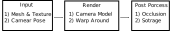
\includegraphics[width=\linewidth]{images/synthetic_optical_flow/of_render.pdf}
	\caption{The pipeline of panoramic optical flow rendering.}
	\label{fig:approach:panoof:pipline}
\end{figure}

The synthetic panoramic optical flow rendered with on-the-shelf OpenGL render pipeline and store in the ERP image.
The input are textured 3D mesh and OpenGL's camera pose.
The process shown as the Fig.~\ref{fig:approach:panoof:pipline} composing with the following 3 steps:

\begin{enumerate}
	\item Camera Model: OpenGl render with Equirectangular projection (ERP);
	\item Warp Around: Processing the warp around at the boundary of image;
	\item Occlusion: estimate the occlusion of optical flow ;
\end{enumerate}

\subsubsection{Camera Model}

The traditional OpenGL rendering pipeline doesn't support the panoramic camera model and optical flow generation.
For synthesising ground truth panoramic RGB images and optical flow, we implement and hire equirectangular perspective camera model.

The equirectangular perspective panoramic camera model render the 3D mesh to  equirectangular images.
To achieve the camera model the OpenGL geometry shaders transform the 3D mesh from Cartesian coordinate system to spherical coordinate system. 
The camera mode

Furthermore, we use Replica to demonstrate. 
The Replica dataset coordinate system show as the Fig.~\ref{fig:approach:coord_hotel_00}.

\begin{figure}[hbt!]
	\centering
	\includegraphics[width=\linewidth]{images/synthetic_optical_flow/coord_hotel_00.png}
	\caption{A boat.}
	\label{fig:approach:coord_hotel_00}
\end{figure}

And the coordinate system used in geometry OpenGL shader shown as Fig.~\ref{fig:approach:geometry_cs}.
The forward is $+z$, up is $+y$ and left is $+x$.
Meanwhile, the $\theta$ and 

\begin{figure}[hbt!]
	\centering
	\includegraphics[width=\linewidth]{images/synthetic_optical_flow/coord_hotel_00.png}
	\caption{A boat.}
	\label{fig:approach:geometry_cs}
\end{figure}



\section{Dataset}\label{sec:exp:data}

It's very hard to measure the real word optical flow information, especially the equirectangular image. 
And currently do not have any public optical flow equirectangular image dataset.
So we evaluate our method estimated optical flow quantity in the synthetic equirectangular optical flow dataset.
Meanwhile to analysis the performance we use SSIM e.t.c metrics to evaluate the optical flow warped the equirectangular image sequence in both real world dataset and synthetic dataset.


\subsection{Synthetic Dataset}\label{sec:exp:data:syn}

The rasterization render method OpenGL used to synthesize the ground truth optical flow.
The equirectangular optical flow generation algorithm introduction in Section. \ref{sec:app:panoof}.
Few public indoor 3D datasets are hired to render the ground truth data.

Although, the 3D computer graphics software toolsets, e.g. Blender have functions to estimate the object motion information, e.g motion vector of Blender. 
The rendered object motion used for motion blur e.t.c VFX is not accurate enough. 
There are obviously artefacts at the boundary of moving objects, Figure. ~\ref{fig:exp:blendermv}. 

\begin{figure}[hbt!]
	\centering
	\includegraphics[width=\linewidth]{example-image-a}
	\caption{Blender Motion Vector}
	\label{fig:exp:blendermv}
\end{figure}

\textbf{Replica 360} ~\cite{replica19arxiv}



\textbf{Matterport3D} ~\cite{Matterport3D}


\subsection{Real World Dataset}

We test our method on the real world dataset with warped image sequence.

\section{Comparison}

We compare our method with following state of the art methods, FlowNet2~\cite{ilg2017flownet}, Dense Inverse Search (DIS) optical flow~\cite{kroeger2016fast} and PWC-Net~\cite{sun2018pwc}. 
The FlowNet2~\cite{ilg2017flownet} implementation is NVIDIA official release code \href{https://github.com/NVIDIA/flownet2-pytorch}{flownet2-pytorch}.
The PWC-Net~\cite{sun2018pwc}'s code is \href{https://github.com/NVlabs/PWC-Net}{NVlabs/PWC-Net}

\subsection{Quantity Analysis}

The metrics AAE, EPE and RMS is used for the quantity analysis.

The average endpoint error (\textbf{EPE}):  ~\cite{??}
EPE is the absolute error of all the pixels. 

\begin{equation}\label{equ_exp_epe}
E_{EPE} = \frac{1}{n} \sum_{i \in \Omega}\sqrt{(u_e^i - u_g^i)^2 + (v_e^i - v_g^i)^2}
\end{equation}

The average angular error (\textbf{AAE}):~\cite{??}
AAE is a metric to measure the deviation of angle:

\begin{equation}\label{equ_exp_aae}
	E_{AAE} = \frac{1}{n} \sum_{i \in \Omega}arctan(\frac{u^i_e v^i_g - u^i_g v^i_e}{u^i_e u^i_g + v^i_e v^i_g})
\end{equation}

The root mean square error (\textbf{RMSE}):~\cite{??}

\begin{equation}\label{equ_exp_rmse}
	E_{RMSE} = \sqrt{\frac{1}{n} \sum_{i \in \Omega}((u_e^i - u_g^i)^2 + (v_e^i - v_g^i)^2)}
\end{equation}

The ERP images introduce exaggerated distortion at north and south poles, which make a central angle error at spherical coordinate system in poles have much larger then the equator's.
To evaluate the error with same metric on the whole images, we extend EPE, AAE adn RMS to the spherical coordinate. 
Replace the euclidean distance and angle with the great circle distance (geodesics) and the angles of a spherical triangle. 
The error in spherical coordinate denote with $EPE_{cs}$, $AAE_{cs}$ and $RMS_{cs}$.

The error in spherical coordinate shown as Tab. ~\ref{fig:exp:quality}.



\begin{table}[h!]
	\centering
	\begin{tabular}{ c | c | c | c | c | c | c }
		\hline
		& \multicolumn{6}{c}{DIS}  \\
		\hline
		& ${AAE}$ & ${EPE}$ & ${RMS}$ & ${AAE_{cs}}$ & ${EPE_{cs}}$ & ${RMS_{cs}}$ \\
		\hline
		apartment\_0 & - & - & -  & - & - & -  \\ 
		\hline
		hotel\_0 & - & - & -  & - & - & -  \\ 
		\hline
		office\_0 & - & - & - & - & - & -  \\ 
		\hline
		office\_4 & - & - & -  & - & - & -  \\ 
		\hline
		room\_0 & - & - & - & - & - & -  \\ 
		\hline
		room\_1 & - & - & -  & - & - & -  \\ 
		\hline\hline
		& \multicolumn{6}{c}{Flownet2} \\
		\hline
		& ${AAE}$ & ${EPE}$ & ${RMS}$ & ${AAE_{cs}}$ & ${EPE_{cs}}$ & ${RMS_{cs}}$ \\
		\hline
		apartment\_0 & - & - & -  & - & - & -  \\ 
		\hline
		hotel\_0 & - & - & -  & - & - & -  \\ 
		\hline
		office\_0 & - & - & - & - & - & -  \\ 
		\hline
		office\_4 & - & - & -  & - & - & -  \\ 
		\hline
		room\_0 & - & - & - & - & - & -  \\ 
		\hline
		room\_1 & - & - & -  & - & - & -  \\ 
		\hline\hline
		& \multicolumn{6}{c}{PWCNet} \\
		\hline
		& ${AAE}$ & ${EPE}$ & ${RMS}$ & ${AAE_{cs}}$ & ${EPE_{cs}}$ & ${RMS_{cs}}$ \\
		\hline
		apartment\_0 & - & - & -  & - & - & -  \\ 
		\hline
		hotel\_0 & - & - & -  & - & - & -  \\ 
		\hline
		office\_0 & - & - & - & - & - & -  \\ 
		\hline
		office\_4 & - & - & -  & - & - & -  \\ 
		\hline
		room\_0 & - & - & - & - & - & -  \\ 
		\hline
		room\_1 & - & - & -  & - & - & -  \\ 
		\hline\hline
		& \multicolumn{6}{c}{RAFT} \\
		\hline
		& ${AAE}$ & ${EPE}$ & ${RMS}$ & ${AAE_{cs}}$ & ${EPE_{cs}}$ & ${RMS_{cs}}$ \\
		\hline
		apartment\_0 & - & - & -  & - & - & -  \\ 
		\hline
		hotel\_0 & - & - & -  & - & - & -  \\ 
		\hline
		office\_0 & - & - & - & - & - & -  \\ 
		\hline
		office\_4 & - & - & -  & - & - & -  \\ 
		\hline
		room\_0 & - & - & - & - & - & -  \\ 
		\hline
		room\_1 & - & - & -  & - & - & -  \\ 
		\hline
	\end{tabular}
	\caption{Error of Replica dataset}
	\label{fig:exp:quality}
\end{table}


%\begin{tikzpicture}
%	% Read the file
%	% if needed, define column separators by pgfplotstableread[col sep=...]{}{}
%	\pgfplotstableread{data.csv}{\Data}
%	\begin{groupplot}[
%			group style = {group size = 2 by 1},
%			height = 10cm,
%			width = 10cm,
%			ymin = 500,
%			xticklabels from table = {\Data}{Day}, xtick = {1,...,19},
%			xticklabel style = {rotate = 90, xshift = -0.8ex, anchor = mid east}
%		]
%		\nextgroupplot[xmin = 1, xmax = 19, ymax = 900]
%		\addplot[very thick] table [x = Number, y = Orders] {\Data};
%	\end{groupplot}
%\end{tikzpicture}



\subsection{Quality Analysis}





